
\section{辛不动点的阿诺德猜想}
\label{sec:arnold-conjecture}

在\trCelestialMechanics{}的\trRestrictedThreeBodyProblem{}中寻找%
\trPeriodicSolution{}时，H.~\trPoincare{}在\trEnergySurface{}上构造了一个%
\trAnnulus{} $A$ 的保面积\trSection\trMapping。该\trAnnulus{}以所谓的%
顺行与逆行\trPeriodicOrbit{}为\trBoundary。这促使他在 1912 年表述了下述%
定理 [177]。它称为庞加莱最后几何定理，是他在去世前不久宣布的。它后来由%
G.~\trBirkhoff{}证明。

\begin{theorem}[\trPoincare-\trBirkhoff]\label{thm:poincare-birkhoff}
\trAnnulus{} $A:=S^{1}\times[a,b]$ 上每个保面积且保定向的%
\trHomeomorphism，只要它把两条\trBoundary{}向相反的方向旋转，就在其%
\trInterior{}至少拥有 $2$ 个\trFixedPoint{}（图 6.1）。
\end{theorem}

\noindent\begin{minipage}{\linewidth}
\centering
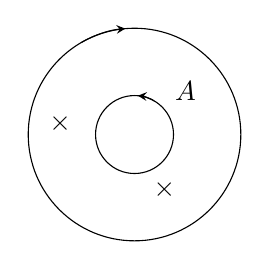
\begin{tikzpicture}[>=stealth,scale=0.9]
  \draw (0,0) circle (1.5);%
  \draw (0,0) circle (0.55);%
  \draw[->] (120:1.5) arc(120:95:1.5);%
  \draw[->] (60:0.55) arc(60:85:0.55);%
  \node at (0.72,0.62) {$A$};%
  \node at (-1.05,0.15) {$\times$};%
  \node at (0.42,-0.78) {$\times$};%
\end{tikzpicture}

图 6.1
\end{minipage}

这个定理的力度在于：一旦把它应用于迭代，它便立刻给出无穷多个%
\trPeriodic{}点，%
这在应用中导致无穷多个\trPeriodicSolution，参见 [24]。1913 年，%
G.~\trBirkhoff{} [23] 以一个精巧但严格二维的论证成功地证明了这个定理。%
注意，这个定理就其本性而言是整体的：对映射不要求任何\trInterior{}假设。%
它不是%
一个拓扑的结果：若去掉保面积假设，它便不成立。S.~\trLefschetz{}本无疑很乐于%
向\trBirkhoff{}演示：著名的\trPoincare-\trBirkhoff\trFixedPoint{}定理不过%
是他自己的拓扑\trFixedPoint{}理论的一个平凡推论，但他不得不承认失败：%
由于\trAnnulus{}的\trEulerCharacteristic{}为零，$\chi(A)=0$，他的理论%
在这里%
用不上。

二维\trSphere{}的\trEulerCharacteristic{}（$\chi(S^{2})=2$）不为零，于是%
按莱夫%
谢茨的理论，$S^{2}$ 上每个与\trIdentityMap\trHomotopic{}连续映射 $f$%
至少拥有一个\trFixedPoint，这当然是众所周知的。映射 $f$ 也可能只有一个%
\trFixedPoint，例如\trRiemann{}\trSphere{}上的平移 $z\mapsto z+1$ 便%
表明了这一点：它唯一%
的\trFixedPoint{}是 $\infty$ 处的北极。

\noindent\begin{minipage}{\linewidth}
\centering
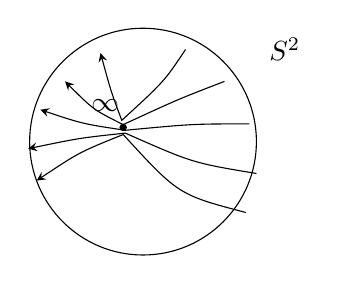
\begin{tikzpicture}[>=stealth,scale=0.9]
  \draw (0,0) circle (1.6);%
  \node at (2.0,1.3) {$S^{2}$};%
  \fill (-0.28,0.2) circle (1.5pt);
  \node[anchor=south east] at (-0.2,0.28) {$\infty$};
  \draw[->] (1.45,-1.0) .. controls (0.5,-0.75) .. (-0.28,0.1)
        .. controls (-0.9,-0.15) .. (-1.5,-0.55);%
  \draw[->] (1.6,-0.45) .. controls (0.7,-0.3) .. (-0.25,0.12)
        .. controls (-0.9,0.05) .. (-1.62,-0.1);%
  \draw[->] (1.5,0.25) .. controls (0.7,0.25) .. (-0.25,0.16)
        .. controls (-0.85,0.25) .. (-1.45,0.45);%
  \draw[->] (1.15,0.85) .. controls (0.5,0.6) .. (-0.28,0.24)
        .. controls (-0.7,0.45) .. (-1.1,0.85);%
  \draw[->] (0.6,1.3) .. controls (0.3,0.85) .. (-0.3,0.3)
        .. controls (-0.45,0.7) .. (-0.6,1.25);%
\end{tikzpicture}

图 6.2
\end{minipage}

然而，一个令人惊叹的事实是：若 $f$ 还是保面积的，它便至少拥有 $2$ 个%
\trFixedPoint。

\begin{theorem}[N.~\trNikishin、C.~\trSimon，1974]\label{thm:nikishin-simon}
$S^{2}$ 的与\trIdentityMap\trHomotopic{}且保持\trRegular\trMeasure{} $\mu$%
的\trHomeomorphism{} $f$ 至少拥有 $2$ 个\trFixedPoint。特别地，$S^{2}$ 的%
每个使面积形式保持不变（$f^{*}\omega=\omega$）的\trDiffeomorphism{}至少%
拥有 $2$ 个\trFixedPoint。
\end{theorem}

\begin{proof}
第二个陈述是第一个陈述的推论。的确，该映射的\trDegree{}为 $1$，从而由%
H.~\trHopf{}定理它与\trIdentityMap\trHomotopic。为证第一个陈述，设%
$P^{*}\in S^{2}$ 是\trLefschetz{}理论所保证的 $f$ 的那个\trFixedPoint。于是%
映射 $g:=f\bigl|_{(S^{2}\setminus P^{*})}$ 可等同于平面 $\R^{2}$ 的一个%
\trHomeomorphism。若 $g$ 没有\trFixedPoint，则由\trBrouwer{}平移定理，会%
存在一个\trOpenSet{} $D$，使得诸 $g^{j}(D)=f^{j}(D)$ 对一切 $j>0$ 相互%
\trDisjoint。但这样一来，由于 $f$ 保持\trMeasure，
\[
\sum_{j=0}^{n}\mu\bigl(f^{j}(D)\bigr)=(n+1)\,\mu(D)\leq\mu\bigl(S^{2}\bigr),
\]
对每个整数 $n\geq1$ 成立，从而 $\mu(D)=0$。这与「$\mu(U)$ 对\trOpenSet{}%
$U$ 不为零」的假设相矛盾。
\end{proof}

\trBrouwer{}平移定理是一个非常特殊的二维现象，曾吸引众多数学家的注意%
[33, 34, 80, 101, 109, 141, 206]。与\cref{thm:nikishin-simon}中相同的%
论证——C.~\trLoewner{}在二十世纪六十年代斯坦福的讲学中曾使用过——也表明：%
平面上开\trDisc{}的\trMeasurePreserving\trHomeomorphism{}总拥有至少一个%
\trFixedPoint。%
若该\trHomeomorphism{}不保持\trRegular\trMeasure，这一点显然不成立。%
上面的定理，其 C.~\trSimon [200] 与 N.~\trNikishin [169] 的证明用的是另一种论证。%
他们证明了：平面上保面积\trDiffeomorphism{}的\trFixedPoint{}指数 $j(P)$%
不超过 $1$。于是，\trFixedPoint{}公式 $\chi(S^{2})=\sum j(P)$ 便要求至少%
$2$ 个\trFixedPoint。

V.~\trArnold{}在 [11] 中观察到：\trPoincare-\trBirkhoff{}结果可以从二维%
\trTorus{} $T^{2}=\R^{2}/\Z^{2}$ 的一个\trFixedPoint{}定理导出，这个%
\trTorus{}是把两个相同的\trAnnulus{}沿其\trBoundary{}粘合起来而构成的；%
细节参见 [46]。

\noindent\begin{minipage}{\linewidth}
\centering
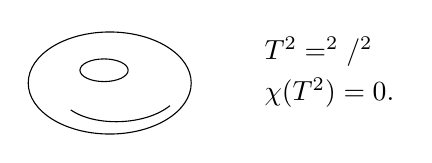
\begin{tikzpicture}[>=stealth,scale=0.9]
  \draw (0,0) ellipse (1.15 and 0.72);%
  \draw (-0.08,0.18) ellipse (0.34 and 0.16);%
  \draw (-0.55,-0.38) .. controls (-0.2,-0.62) and (0.5,-0.6) .. (0.85,-0.32);%
  \node[align=left] at (3.1,0.15) {$T^{2}=\R^{2}/\Z^{2}$\\[3pt] $\chi(T^{2})=0$.};
\end{tikzpicture}

图 6.3
\end{minipage}

与 $S^{2}$ 相对照，\trLefschetz\trFixedPoint{}理论恰恰对这个\trSurface{}不%
适用，因为 $\chi(T^{2})=0$。的确，\trTorus{}上存在没有\trFixedPoint{}的%
保面积%
\trDiffeomorphism，覆盖空间 $\R^{2}$ 上由
\begin{equation}\label{eq:torus-translations}
X=x+c_{1},\qquad Y=y+c_{2},
\end{equation}
给出的诸\trTranslation{}映射便表明了这一点。因此，若要求它们拥有%
\trFixedPoint，%
$T^{2}$ 上\trSymplectic\trMapping{}的类就必须加以限制。我们循着%
V.~\trArnold，考察 $T^{2}$ 的与\trIdentityMap\trHomologous%
\trMeasurePreserving%
\trDiffeomorphism{} $\psi$；从而它们在 $\R^{2}$ 上由%
$\psi:(x,y)\mapsto(X,Y)$ 给出：
\begin{equation}\label{eq:torus-lift-form}
\begin{aligned}
X\ &=\ x+p(x,y)\\
Y\ &=\ y+q(x,y)
\end{aligned}
\end{equation}
其中 $p$ 与 $q$ 是\trPeriodic{}函数，我们还要求 $\psi$ 保持%
\textbf{\trCenterOfMass}（center of mass），从而特别地把诸平移排除在外。总括起来，%
$T^{2}$ 的\trDiffeomorphism{} $\psi$ 须满足下列条件
\begin{align*}
\text{(i)}\qquad&\ \text{$\psi$ 与恒同映射\trHomologous}\\
\text{(ii)}\qquad&\ dX\wedge dY=dx\wedge dy\\
\text{(iii)}\qquad&\ \int_{T^{2}}p=0=\int_{T^{2}}q.
\end{align*}

\begin{proposition}\label{prop:torus-fixed-points}
$T^{2}$ 的满足 (i)--(iii) 的\trDiffeomorphism{} $\psi$，只要它充分接近%
\trIdentityMap{}（按 $C^{1}$ \trNorm），便拥有 $\geq3$ 个\trFixedPoint。%
此外，若全部\trFixedPoint{}都\trNondegenerate，则 $\psi$ 拥有 $\geq4$ 个%
\trFixedPoint。
\end{proposition}

\begin{proof}
由于 $\psi:(x,y)\mapsto(X,Y)$ 充分接近\trIdentityMap，它可以由一个以隐%
形式给出的\trGeneratingFunction{} $F:\R^{2}\to\R$ 表示：
\begin{equation}\label{eq:torus-generating}
\begin{aligned}
X\ &=\ x+\frac{\partial F}{\partial Y}(x,Y)\\
y\ &=\ Y+\frac{\partial F}{\partial x}(x,Y),
\end{aligned}
\end{equation}
参见附录 A.1。$F$ 的\trGradient{}是\trPeriodic{}的，而由假设 (iii) 可知%
函数 $F$ 本身也是\trPeriodic{}的，因而是 $T^{2}$ 上的一个函数。我们从%
\eqref{eq:torus-generating} 得知：$\psi$ 在 $T^{2}$ 上的诸\trFixedPoint{}%
与函数 $F$ 在 $T^{2}$ 上的诸\trCriticalPoint{}一一对应。按%
\trLjusternik-\trSchnirelman{}理论，二维\trTorus{}上的每个\trSmooth{}%
函数至少拥有 $3$ 个\trCriticalPoint{}（见下文 6.3 节）；而按%
\trMorseTheory，若先验地知道全部\trCriticalPoint{}都\trNondegenerate，%
则它至少拥有 $4$ 个\trCriticalPoint。命题得证。
\end{proof}

当然，$T^{2}$ 上存在恰有 $3$ 个\trFixedPoint{}的\trSymplectic{}映射，%
甚至有接近\trIdentityMap{}的。为此，我们取 $T^{2}$ 上一个恰有 $3$ 个%
\trCriticalPoint{}的\trSmooth{}函数。这类函数的一个例子是
\[
G(x,y)=\sin\pi x\cdot\sin\pi y\cdot\sin\pi(x+y),
\]
其水平线如图 6.4\footnote{原书图注印作「$T^{2}=\R^{2}/\,2\pi\Z^{2}$」，与本节%
通篇的 $T^{2}=\R^{2}/\Z^{2}$ 约定不合（参见图 6.3；随后的例子%
$G(x,y)=\sin 2\pi x+\sin 2\pi y$ 也以 $1$ 为周期），疑为衍余「$2\pi$」之误，%
图中径改。——译者注}所示。

\noindent\begin{minipage}{\linewidth}
\centering
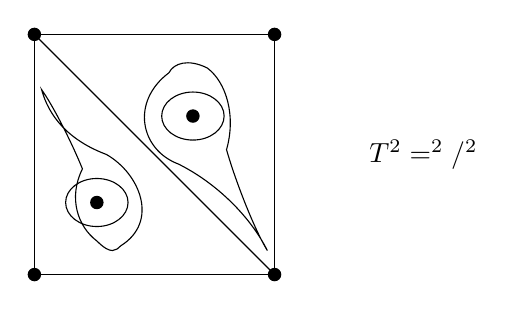
\begin{tikzpicture}[>=stealth,scale=3.05]
  \draw (0,0) rectangle (1,1);%
  \draw (0,1) -- (1,0);%
  \fill (0.66,0.66) circle (0.028);%
  \fill (0.26,0.30) circle (0.028);%
  \draw (0.66,0.66) ellipse (0.13 and 0.10);%
  \draw (0.56,0.84) .. controls (0.40,0.72) and (0.44,0.52) .. (0.60,0.46)
        .. controls (0.76,0.38) and (0.90,0.24) .. (0.97,0.10)
        .. controls (0.92,0.18) and (0.84,0.38) .. (0.80,0.52)
        .. controls (0.84,0.66) and (0.80,0.80) .. (0.72,0.86)
        .. controls (0.64,0.90) and (0.58,0.88) .. (0.56,0.84);%
  \draw (0.26,0.30) ellipse (0.13 and 0.10);%
  \draw (0.36,0.12) .. controls (0.52,0.22) and (0.44,0.42) .. (0.30,0.50)
        .. controls (0.14,0.56) and (0.06,0.66) .. (0.03,0.77)
        .. controls (0.08,0.70) and (0.16,0.54) .. (0.20,0.44)
        .. controls (0.14,0.32) and (0.18,0.20) .. (0.26,0.14)
        .. controls (0.32,0.08) and (0.34,0.10) .. (0.36,0.12);%
  \fill (0,0) circle (0.028);\fill (1,0) circle (0.028);
  \fill (0,1) circle (0.028);\fill (1,1) circle (0.028);
  \node[align=left] at (1.62,0.5) {$T^{2}=\R^{2}/\Z^{2}$};
\end{tikzpicture}

图 6.4
\end{minipage}

$G$ 在左三角形中有一个最大点，在右三角形中有一个最小点，而在单位正方形的%
诸角点处有一个\textbf{\trMonkeySaddle}（monkey saddle）。若 $\varepsilon>0$ 充分小，%
我们以 $F=\varepsilon G$ 为\trGeneratingFunction，由%
\eqref{eq:torus-generating} 隐式地定义映射 $\psi:(x,y)\to(X,Y)$。于是%
$\psi$ 接近\trIdentityMap，满足 (i)--(iii)，并且拥有 $3$ 个\trFixedPoint，%
即 $G$ 在 $T^{2}$ 上的诸\trCriticalPoint。类似地，函数%
$G(x,y)=\sin 2\pi x+\sin 2\pi y$ 定义了一个在 $T^{2}$ 上拥有 $4$ 个%
\trFixedPoint{}的映射 $\psi$，它们全都\trNondegenerate。\quad$\blacksquare$

把\trSymplectic\trMapping{}的诸\trFixedPoint{}与一个相配函数的诸%
\trCriticalPoint{}联系起来，这一思想可追溯到 H.~\trPoincare{} [176]，%
而且常被用来建立局部存在性结果。例如，A.~\trWeinstein{} [222, 224] 利用%
它证明了：\trCompact{}且\trSimplyConnected{}的\trSymplecticManifold{} $M$%
的\trSymplecticDiffeomorphism，只要接近\trIdentityMap，其\trFixedPoint{}%
就至少与 $M$ 上一个函数的\trCriticalPoint{}一样多。更一般的结果与文献，%
参见 J.~\trMoser{} [165]。与所有这些\trPerturbation{}结果形成鲜明对照的%
是，我们现在要转向的\trArnold{}猜想对任意\trSymplectic\trMapping{}索求%
\trFixedPoint。对 $T^{2}$ 这一特殊情形，V.~\trArnold{}在 [10] 中猜想：%
\cref{prop:torus-fixed-points} 在没有「$\psi$ 接近\trIdentityMap」这一%
限制性假设时仍然成立。

为了引入适用于\trFixedPoint{}理论的那个受限\trSymplecticDiffeomorphism{}%
类，我们先指出：对 $T^{2}$ 上的\trDiffeomorphism{} $\psi$，假设%
(i)--(iii) 等价于要求 $\psi$ 属于 $T^{2}$ 上某个\trTimeDependent%
\trHamiltonianVectorField{} $X_{H}$ 的\trFlow。其证明并不容易，参见%
C.~\trConley{}与 E.~\trZehnder{} [55]。于是，依据下述\trhDefinition，%
$\psi$ 是%
$T^{2}$ 的一个\textbf{\trHamiltonianMap}（Hamiltonian map）：

\begin{definition}\label{def:hamiltonian-map}
设 $(M,\omega)$ 是一个\trSymplecticManifold。$M$ 的\trDiffeomorphism{}%
$\psi$ 称为\trHamiltonian{}的，如果它属于 $M$ 上某个\trTimeDependent%
\trHamiltonianVectorField{} $X_{H}$ 的\trFlow。更精确地说：存在\trSmooth{}%
函数 $H:S^{1}\times M\to\R$，使得 $\psi=\varphi^{1}$，其中 $M$ 的%
\trSymplecticDiffeomorphism{}族 $\varphi^{t}$（$t\in\R$）满足
\begin{align*}
\frac{d}{dt}\,\varphi^{t}\ &=\ X_{H}\bigl(\varphi^{t}\bigr)\\
\varphi^{0}\ &=\ \id.
\end{align*}
\end{definition}

在其博士论文中，A.~\trBanyaga [16] 证明了：映射 $\psi$ 是一个%
\trHamiltonianMap，当且仅当它属于 $M$ 的\trSymplecticDiffeomorphism{}群%
之恒同分支的\trCommutator{}子群。此外，他还证明了 $\psi$ 是%
\trHamiltonian{}的当且仅当 $\psi$ 的\trCalabi{}不变量为零。%
\trHamiltonianMap{}与\trIdentityMap\trHomotopic，故按\trLefschetz{}的理论，%
只要\trEulerCharacteristic{} $\chi(M)$ 不为零，它当然拥有\trFixedPoint。

\textbf{\trArnold{}猜想。}\quad \trCompact\trSymplecticManifold{}%
$(M,\omega)$ 的每个\trHamiltonianDiffeomorphism{} $\psi$ 所拥有的%
\trFixedPoint，至少与 $M$ 上函数 $F:M\to\R$ 所可能具有的最少%
\trCriticalPoint{}数一样多。

鉴于 $M$ 上函数的\trLjusternik-\trSchnirelman{}理论与\trMorseTheory，%
我们把这个猜想以如下稍弱的形式重新表述：
\[
\#\{\ \text{$\psi$ 的\trFixedPoint}\ \}\ \geq\ \text{$M$ 的\trCupLength}+1\,,
\]
而若先验地知道 $\psi$ 的诸\trFixedPoint{}皆\trNondegenerate，则
\[
\geq\ \text{$M$ 的\trBettiNumber{}之和}\,.
\]

回顾：$\psi$ 的\trFixedPoint{} $p$ 称为\trNondegenerate{}的，如果 $1$ 不%
是\trLinearization{}映射 $d\psi(p)\in L(T_{p}M)$ 的\trEigenvalue。%
\trManifold{} $M$%
的\textbf{\trCupLength}（cup-length）定义为\trCohomology{}环中最长的乘积：
\begin{align*}
CL(M)=\sup\bigl\{\,k\ \bigm|\ \exists\ \alpha_{1},\alpha_{2},\ldots,%
\alpha_{k}\in H^{*}(M),\ \dim\alpha_{j}\geq1\ \text{使得}\\
\alpha_{1}\cup\alpha_{2}\cup\cdots\cup\alpha_{k}\neq0\,\bigr\}.
\end{align*}
以 $SB(M)$ 表示 $M$ 的\textbf{\trBettiNumber}（Betti numbers）之和，其中%
$\beta_{k}=\dim H^{k}(M)$（$0\leq k\leq\dim M$）。引入\trPoincare{}多项式
\[
P(t,M)=\sum_{k=0}^{\dim M}\beta_{k}\,t^{k},\qquad \beta_{k}=\dim H^{k}(M)
\]
我们便有 $SB(M)=P(1,M)$，当然还有 $P(-1,M)=\chi(M)$，后者即 $M$ 的%
\trEulerCharacteristic。在 $2n$ 维\trTorus{} $T^{2n}$ 这一特殊情形，这些%
\trTopology\trInvariant{}量为 $CL(T^{2n})=2n$ 与 $SB(T^{2n})=2^{2n}$，而%
$\chi(T^{2n})=0$。%
特别地，对\cref{prop:torus-fixed-points}中的 $T^{2}$，我们看到%
$3=CL(T^{2})+1$ 与 $4=SB(T^{2})$。

我们更愿意把这一猜想用\trDynamics{}的方式重新表述。按定义，%
\trHamiltonianMap{} $\psi$ 是 $M$ 上\trHamiltonianEquation{}%
$\dot{x}=X_{H}(x)$ 之\trFlow{}的\trTimeOneMap，此处\trSmooth{}函数%
$H:\R\times M\to\R$ 关于时间%
\trPeriodic：$H(t+1,x)=H(t,x)$。于是，$p$ 是 $\psi$ 的\trFixedPoint{}当且%
仅当 $p=x(0)$ 是\trHamiltonianEquation{}的某个解 $x(t)$ 的初始条件，该解%
以 $1$ 为\trPeriodic，从而对一切 $t\in\R$ 满足 $x(t+1)=x(t)$。这样的解%
也称为%
一个\trForcedOscillation。我们与其寻找映射的\trFixedPoint，不如同样去%
寻找\trTimeDependent\trHamiltonianVectorField{}的诸\trPeriodicSolution；%
\trArnold{}猜想给出的，正是以\trSymplecticManifold{}的诸\trTopology%
\trInvariant{}量来表示的\trForcedOscillation{}数目的一个\trUniversal{}%
下界。

若 $(M,\omega)$ 是\trCompact\trSymplecticManifold{}，且%
$H:\R\times M\to\R$ 是满足 $H(t+1,x)=H(t,x)$ 的\trSmooth{}时间%
\trPeriodic{}函数，则对\trTimeDependent\trHamiltonianEquation
\[
\dot{x}=X_{H}(x),\qquad x\in M
\]
下述结论成立：
\[
\#\{\ \text{可缩的}\ 1\text{-\trPeriodicSolution}\ \}\ \geq\ CL(M)+1.
\]
\[
\bigl(\ \geq\ SB(M)\ \text{若诸可缩的}\ 1\text{-\trPeriodicSolution}\ %
\text{皆\trNondegenerate}\ \bigr).
\]

此处一个\trPeriodicSolution{} $x$ 称为\trNondegenerate{}的，如果 $1$ 不是%
$x$ 的\trFloquet{}乘子。由于对函数 $H$ 没有作任何假设，我们只寻找可缩的%
诸\trPeriodicSolution。的确，若\trHamiltonianVectorField{}很小，则%
$1$-\trPeriodicSolution{} $x(t)$ 的弧长就很小，从而该\trOrbit{}必定可缩。%
这由公式
\[
\operatorname{length}(x)=\int_{0}^{1}\bigl|\dot{x}(t)\bigr|\,dt
=\int_{0}^{1}\bigl|X_{H}\bigl(x(t)\bigr)\bigr|\,dt,
\]
得出，其中我们在 $M$ 上取定了一个\trRiemann{}度量。

现在在\trSymplecticManifold{} $(M,\omega)$ 上取一个满足%
$\omega_{x}(v,Ju)=g_{x}(v,u)$（对一切 $v,u\in T_{x}M$）的%
\trAlmostComplexStructure{} $J$，此处 $g$ 是 $M$ 上的一个\trRiemann{}%
度量。于是 $M$ 上每个\trHamiltonianVectorField{} $X_{H}$ 都形如
\[
\dot{x}=J_{x}\,\nabla H(t,x),\qquad x\in M
\]
其中 $H$ 关于 $x$ 的\trGradient{}借助相配的\trRiemann{}度量 $g$ 来定义。%
现设 $H(t,x)=H(x)$ 不依赖于时间，并且在 $C^{2}$ 意义下充分小。此时每个%
$1$-\trPeriodicSolution{} $x(t)$ 的弧长都很小，故其像足够靠近一点而含于%
一个\trDarboux{}坐标卡之内\footnote{原书印作「$1$-周期解可缩，因而含于%
一个 Darboux 坐标卡之内」；单凭可缩推不出含于单张坐标卡，起作用的实为%
上文之弧长估计——小性使轨道足够短，其像方落入一张坐标卡，可缩系随之%
而来。此处已按此径改。——译者注}（从而可缩）；于是按第 5 章中的%
\cref{prop:autonomous-geodesic}之证明中的论证，%
它必为常值，即 $x(t)\equiv x(0)$。这样一来，$1$-\trPeriodicSolution{}%
恰好就是函数 $H:M\to\R$ 的诸\trCriticalPoint{}，而\trArnold{}猜想在这个%
特殊情形下便化归为\trLjusternik-\trSchnirelman{}与\trMorse{}关于函数%
\trCriticalPoint{}的理论。

对标准\trTorus{} $(T^{2n},\omega_{0})$ 这一特殊情形，\trArnold{}猜想于%
1983 年由 C.~\trConley{}与 E.~\trZehnder{} [55] 证明。其证明基于%
\trForcedOscillation{}的\trAction{}原理。同一原理使得 A.~\trFloer{}%
[82]（1986）与%
J.C.~\trSikorav{} [198]（1985）得以对这个猜想，在容有带非正%
\textbf{\trSectionalCurvature}（sectional curvature）\footnote{原书印作「非负」%
（nonnegative），疑为「非正」（nonpositive）之误，此处径改——亏格 $g\geq2$ 的%
闭定向曲面不可能处处非负曲率，否则与本句随即断言的「包括一切正亏格%
定向曲面」相抵。——译者注}的相容\trRiemann{}结构的大类%
\trSymplecticManifold{}上予以证实。这些类特别包括所有具正%
\textbf{\trGenus}（genus）$g$ 的\trOriented\trSurface{} $S_{g}$。

\noindent\begin{minipage}{\linewidth}
\centering
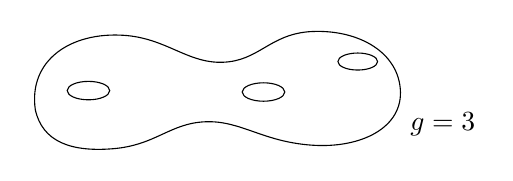
\begin{tikzpicture}[>=stealth,scale=0.9]
  \draw (-2.6,-0.55) .. controls (-2.7,0.15) and (-2.1,0.55) .. (-1.35,0.5)
        .. controls (-0.75,0.46) and (-0.45,0.1) .. (0.05,0.12)
        .. controls (0.55,0.14) and (0.7,0.5) .. (1.25,0.55)
        .. controls (1.9,0.6) and (2.5,0.3) .. (2.55,-0.25)
        .. controls (2.6,-0.8) and (2.0,-1.1) .. (1.3,-1.05)
        .. controls (0.6,-1.0) and (0.3,-0.7) .. (-0.2,-0.72)
        .. controls (-0.7,-0.74) and (-0.9,-1.05) .. (-1.5,-1.1)
        .. controls (-2.1,-1.15) and (-2.5,-1.0) .. (-2.6,-0.55);%
  \draw (-1.85,-0.28) ellipse (0.30 and 0.13);%
  \draw (0.62,-0.30) ellipse (0.30 and 0.13);%
  \draw (1.95,0.13) ellipse (0.28 and 0.12);%
  \node at (3.15,-0.75) {$g=3$};
\end{tikzpicture}

图 6.5
\end{minipage}

\[
CL(S_{g})=3,\qquad SB(S_{g})=2+2g.
\]

更早的证明出于 Ya.~\trEliashberg{}，针对\trSurface{} [77]，基于不同的思想%
且从未%
发表。$S^{2}=\C P^{1}$ 的情形由 B.~\trFortune [93, 94] 于 1985 年推广到更高%
维，他对具标准\trSymplecticStructure{}的 $\C P^{n}$ 验证了这个猜想。%
于是 $\C P^{n}$ 上每个\trHamiltonianMap{}都拥有 $\geq n+1$ 个%
\trFixedPoint。注意，此时 $CL+1=SB=\chi=n+1$，故在\trNondegenerate{}情形，%
这个结果由\trLefschetz{}定理即可得出。A.~\trWeinstein{}在 [227]（1986）中%
指出：若\trHamiltonianMap{} $\psi$ 由一个在 $C^{0}$ \trNorm{}下充分小的%
\trHamiltonianVectorField{}生成，则\trArnold{}猜想对每个%
\trSymplecticManifold{} $(M,\omega)$ 都成立。更晚近的整体结果与发展，%
我们将在本章 6.4 节和 6.5 节中介绍。事实将表明，\trCompact%
\trSymplecticManifold{}上\trHamiltonianVectorField{} $X_{H}$ 的诸%
\trForcedOscillation{}与底\trManifold{} $M$ 的\trTopology{}之间的关联，%
远比上面那个猜想所提示的更为紧密。我们首先详细研究标准\trTorus{}这一%
模型情形。

在转向高维\trArnold{}猜想的证明之前，我们想提一下与%
\trPoincare-\trBirkhoff{}定理相关的一些晚近二维结果。如前所述，二维%
\trTorus{} $T^{2}$ 的\trArnold{}猜想可以看成这个定理对\trDiffeomorphism{}%
的推广，于是人们可以问：是否存在一个拓扑的类似物。就在不久之前，%
P.~\trLeCalvez [139] 成功证明了：$T^{2}$ 的每个与\trIdentityMap%
\trHomotopic、保持\trRegular\trMeasure{}并保持\trCenterOfMass{}（即存在到%
$\R^{2}$ 的提升满足上面 \eqref{eq:torus-lift-form}%
中的条件 (iii)）的\trHomeomorphism{}至少拥有三个\trFixedPoint。更早一些，%
M.~\trFlucher{} [91] 通过扩展 J.~\trFranks{} [96, 97] 的技巧与论证找到了%
两个\trFixedPoint。把这些结果推广到高维\trTorus{}之\trHomeomorphism{}的%
尝试注定失败：在 $T^{n}$（$n\geq3$）上\footnote{原书文本层作 $T^{n}$，页图字形近 $T^{m}$，此处照录原书面貌。——译者注}，存在满足与 $T^{2}$ 情形相类比之%
假设、却没有任何\trFixedPoint{}的\trMeasurePreserving\trDiffeomorphism，%
见%
M.~\trFlucher{} [91]。对\trAnnulus{}的\trPoincare-\trBirkhoff{}定理的一个%
有趣变形，由 J.M.~\trGambaudo{}与 P.~\trLeCalvez [103] 发现，并且独立地由%
J.~\trFranks{} [100] 发现：

\begin{theorem}\label{thm:annulus-infinite-orbits}
\trClosed\trAnnulus{} $A=\R/\Z\times[0,1]$ 的一个\trDiffeomorphism，若与%
恒同\trIsotopic{}且保持\trRegular\trMeasure，则只要它拥有一个%
\trFixedPoint，它在 $A$ 的\trInterior{}就拥有无穷多条\trPeriodicOrbit。
\end{theorem}

这个结果有一些令人惊叹的推论。在一个\trFixedPoint{}的\trNeighborhood{}内%
引入\trPolarCoordinates{} $(r,\vartheta)$，就可以把这个\trFixedPoint{}%
爆破（blow-up）成一条由 $r=0$ 定义的\trInvariant\trCircle。给定 $S^{2}$ 上的两个%
\trFixedPoint，这样就得到一个\trClosed\trAnnulus{}的映射，从而从%
\cref{thm:annulus-infinite-orbits}推出下述：

\textbf{\trhCorollary。}\quad 考虑 $S^{2}$ 的一个保定向且保持%
\trRegular\trMeasure{}的 $C^{2}$-\trDiffeomorphism。若它拥有 $3$ 个%
\trFixedPoint，则它拥有无穷多条\trPeriodicOrbit。

鉴于\cref{thm:nikishin-simon}，这样的\trDiffeomorphism{}总至少拥有两个%
\trFixedPoint，因而只须假设其中之一是\trHyperbolic{}的。的确，一个%
\trHyperbolic\trFixedPoint{}爆破后的\trInvariant\trCircle{}含有 $4$ 个%
\trFixedPoint，故\cref{thm:annulus-infinite-orbits}适用。

J.~\trFranks{}借助\cref{thm:annulus-infinite-orbits}在\trRiemann{}几何的%
一个古老问题上取得了突破。在 [25] 中，G.~\trBirkhoff{}描述了一种把%
带\trRiemann{}度量的二维\trSphere{}上\trGeodesic{}流的研究化归为保面积%
\trAnnulus\trMapping{}之研究的做法，这种映射的诸\trPeriodic{}点对应于%
诸\trClosed\trGeodesic。他证明了：在正\trGauss{}曲率的情形，对应于一条%
简单闭\trGeodesic，这样的\trBirkhoff{}\trAnnulus{}映射是有定义的。%
\trFranks{}假定 $S^{2}$ 装备了一个\trRiemann{}度量，它具有一条使相应的%
\trBirkhoff{}\trAnnulus{}映射有定义的简单闭\trGeodesic；在此假设下%
他证明：该映射拥有一个\trFixedPoint，从而由%
\cref{thm:annulus-infinite-orbits}，拥有无穷多个\trPeriodic{}点。%
另一方面，若 $S^{2}$ 上的一个\trRiemann{}度量没有任何使%
\trBirkhoff{}\trAnnulus{}映射有定义的简单闭\trGeodesic，则%
V.~\trBangert{} [15] 把\trVariational{}方法应用于 $S^{2}$ 的%
\trLoopSpace{}上的\trEnergy\trFunctional，建立了无穷多条%
\trClosed\trGeodesic。众所周知，每个带\trRiemann{}度量的二维\trSphere{}%
都拥有一条简单闭\trGeodesic。于是，带\trRiemann{}度量的二维\trSphere{}上%
总有作为点集互不相同的无穷多条\trClosed\trGeodesic。

与\trPoincare-\trBirkhoff{}定理及其推广相关的文献有：[4, 35, 38, 49, 48, %
61, 91, 95, 96, 97, 98, 99, 103, 109, 138, 140, 141, 139, 200, 206, 143]。
